\section{Benchmarking Aggressive Action and Association}
A$^3$Bench is designed to evaluate fine-grained aggressive action and association in real-world videos. The benchmark construction begins with video curation and structured annotation of aggressive interactions, including actions, participants, roles, and scene context. These annotations are then converted into three levels of diagnostic VQA questions, ranging from basic attribute recognition to compound association and detailed aggressor-action-victim reasoning. The resulting benchmark enables controlled evaluation of MLLMs under a unified multiple-choice protocol.

\begin{table}[t]
    \small
    \centering
    \caption{\textbf{Comparison of A$^3$Bench with prior crime/violence/aggressive action benchmarks.} Cls = action categories. Roles = whether explicit semantic roles (aggressor, victim, bystander) are annotated. Desc. = natural-language person descriptions. Multi-P = multi-person annotation with distinct participants. VQA = structured video question-answer pairs.
    \AB{Draft addressing YSR's comment -- added \# Videos, \# QA, Multi-P columns and abbreviated headings. CABAD/IARD video counts need verification. Remove this note when finalized.}
    }
    \label{tab:benchmark_comparison}
    \resizebox{\textwidth}{!}{
    \begin{tabular}{lcrccccc}
     \toprule
     \textbf{Benchmark} & \textbf{Cls} & \textbf{\# Videos} & \textbf{\# QA} & \textbf{Roles} & \textbf{Desc.} & \textbf{Multi-P} & \textbf{VQA} \\
     \midrule
     DVD \cite{dvd}                  & 2  & 500   & --     & \xmark & \xmark & \xmark & \xmark \\
     Movies Fight \cite{moviesfight} & 2  & 200   & --     & \xmark & \xmark & \xmark & \xmark \\
     RLVS \cite{rlvs}               & 2  & 2,000 & --     & \xmark & \xmark & \xmark & \xmark \\
     RWF-2000 \cite{rwf}            & 2  & 2,000 & --     & \xmark & \xmark & \xmark & \xmark \\
     VID \cite{vid}                  & 2  & 3,020 & --     & \xmark & \xmark & \xmark & \xmark \\
     Violent Flows \cite{rlvs}       & 2  & 246   & --     & \xmark & \xmark & \xmark & \xmark \\
     \midrule
     CABAD \cite{cabad}              & 6  & 483   & --     & \xmark & \xmark & \xmark & \xmark \\
     CRxK \cite{crxk}               & 13 & 3,484 & --     & \xmark & \xmark & \xmark & \xmark \\
     IARD \cite{iard}                & 4  & 804   & --     & \xmark & \xmark & \xmark & \xmark \\
     UCF-Crime \cite{ucfcrimes}      & 14 & 1,900 & --     & \xmark & \xmark & \xmark & \xmark \\
     XD-Violence \cite{xdviolence}   & 7  & 4,754 & --     & \xmark & \xmark & \xmark & \xmark \\
     \midrule
     \textbf{A$^3$Bench (Ours)}      & \textbf{18} & \textbf{2,683} & \textbf{18,748} & \textbf{\cmark} & \textbf{\cmark} & \textbf{\cmark} & \textbf{\cmark} \\
     \bottomrule
    \end{tabular}
    }
\end{table}



\subsection{Construction}
\textbf{Video curation and annotation:}
We curate a benchmark of 2,683 video clips collected from diverse sources, including publicly available social-media videos, UCF-Crime~\cite{ucfcrimes}, and RWF-2000~\cite{rwf}. Source videos are trimmed into shorter clips centered on individual interactions, resulting in an average clip duration of 5.75 seconds. The videos span a wide range of recording conditions, camera viewpoints, resolutions, scene layouts, and levels of visual clutter, reflecting the heterogeneity of real-world scenarios. The final corpus contains 2,234 clips with aggressive behavior and 449 non-aggressive clips.

A group of annotators labeled each video with structured scene information. The annotations include: (1) the aggressive action being performed, selected from 17 aggressive action categories and a control ``none'' category for non-aggressive clips; a short appearance description of the (2) aggressor; (3) victim; (4) bystanders (if any) and (5) the environment or setting. As seen in Figure~\ref{fig:dataset_video_examples}, person descriptions are primarily based on clothing and coarse visual appearance, such as ``person in a dark jacket,'' while avoiding names, faces, demographic attributes, or other identifying information. This design reduces the risk of relying on sensitive attributes and focuses the benchmark on visual role and action understanding. If a certain role does not exist in the video clip, or the appearance is too ambiguous, that is left out in the annotations. More details are provided in Figure~\ref{fig:dataset_demograph} and ~\ref{fig:video_role_count}.


\textbf{Annotation quality assurance:}
We curate A$^3$Bench to ensure visually grounded and reliable annotations for aggressive interactions. Because real-world clips often include occlusion, crowds, similar-looking participants, and ambiguous roles, annotators mark roles at the appropriate specificity, using collective labels or avoiding vague person descriptions when needed. Multiple annotators verify that action labels, participant roles, and aggressor-action-victim relations are supported by observable visual evidence. Unreliable annotations were re-edited through discussion and multiple revision rounds. This process preserves the complexity of real-world footage while improving annotation accuracy and consistency.

\begin{figure}[t]
  \centering
  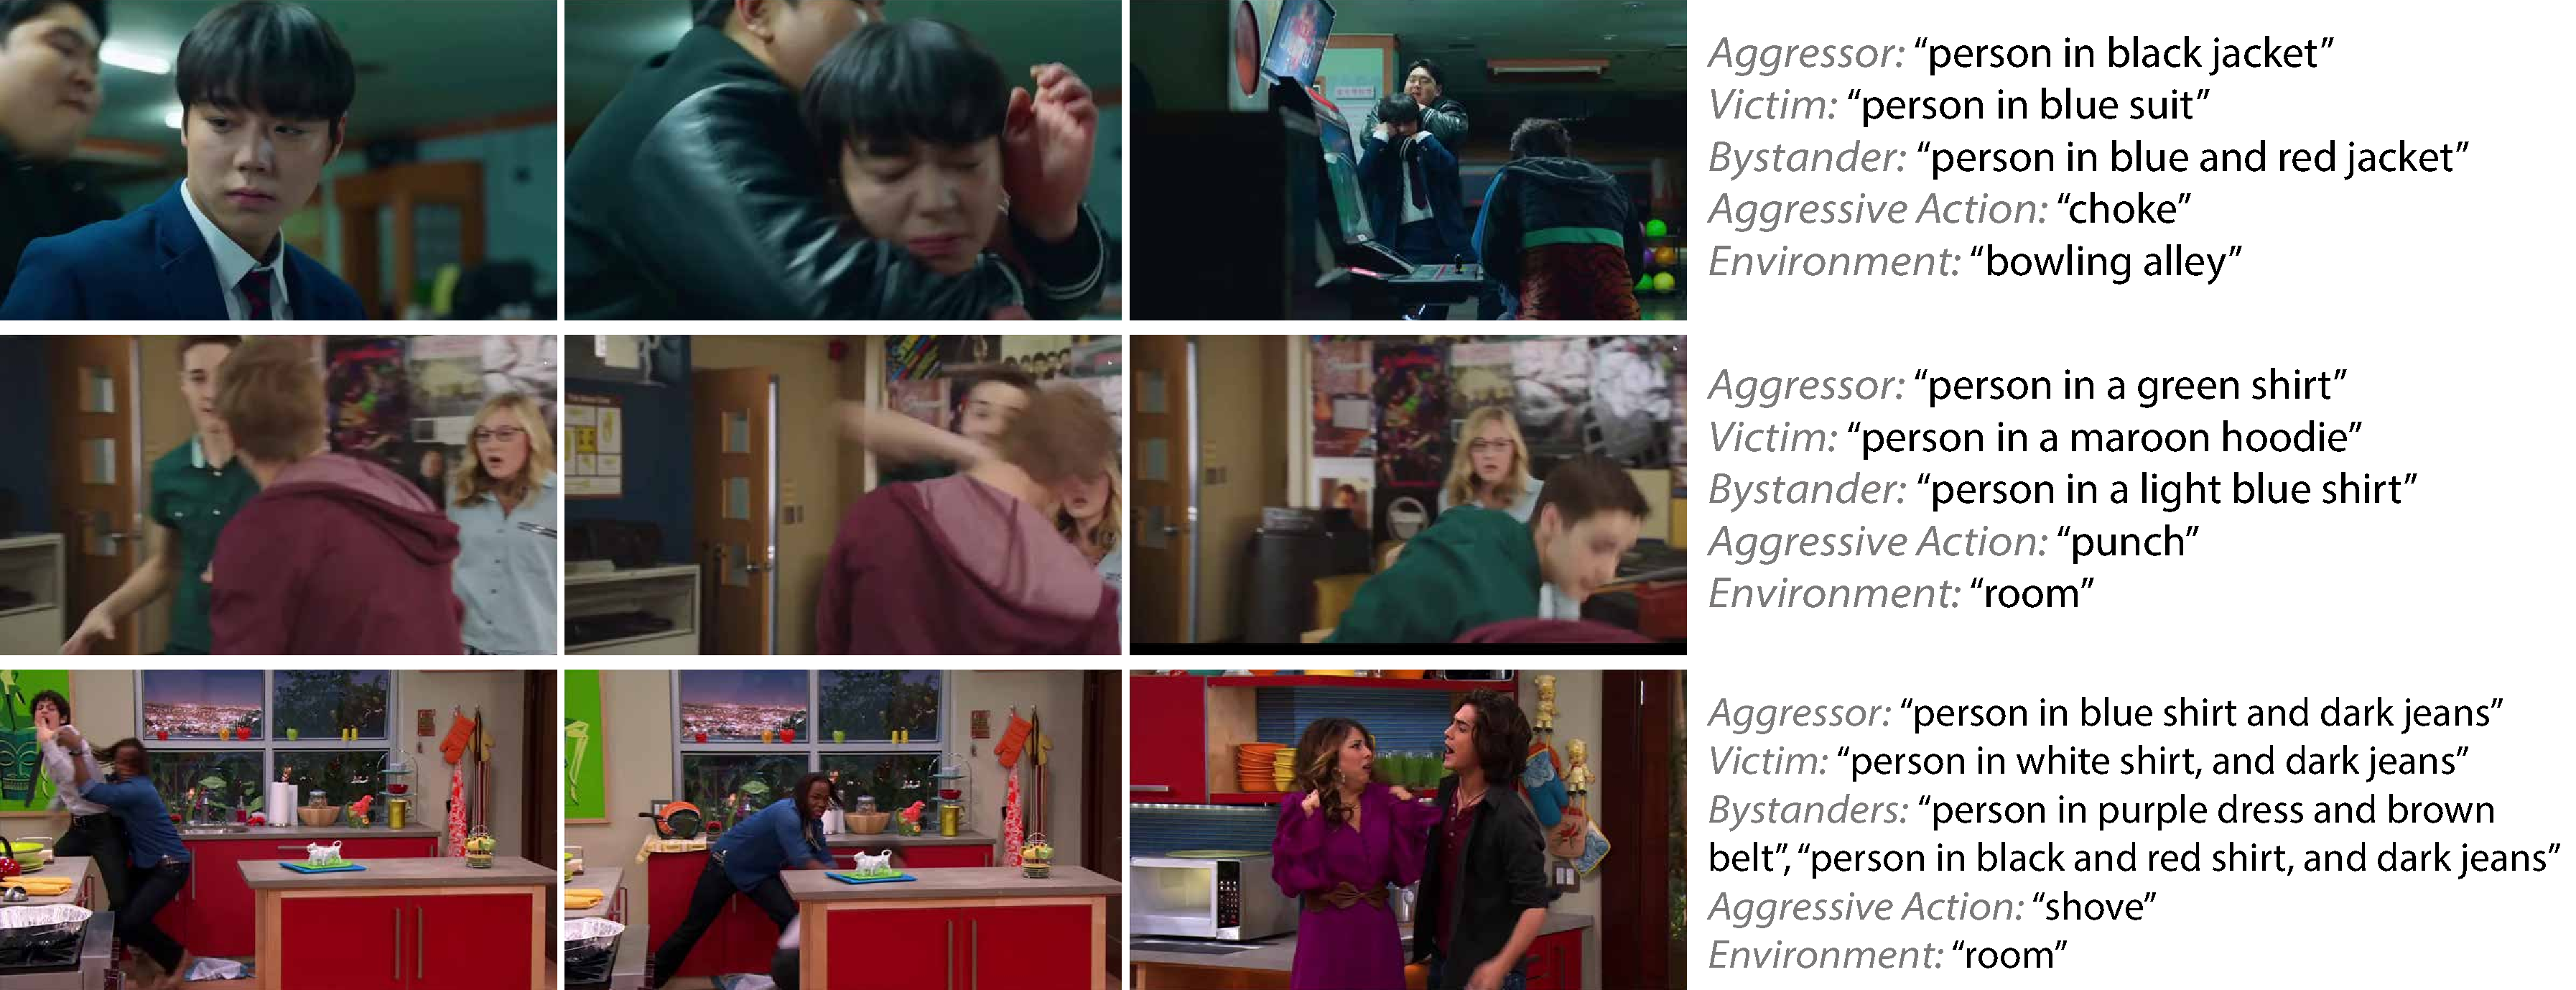
\includegraphics[width=\linewidth]{figures/dataset.pdf}
  \caption{\textbf{Example videos from A$^3$Bench.}
Each video is annotated with structured role and scene information, including the aggressor, victim, bystanders, aggressive action, and environment. Person descriptions are based primarily on clothing and coarse visual attributes rather than identity, enabling fine-grained actor-role association while avoiding personally identifying information.
}
  \label{fig:dataset_video_examples}
\end{figure}


\begin{figure}[t!]
  \centering
    \centering
    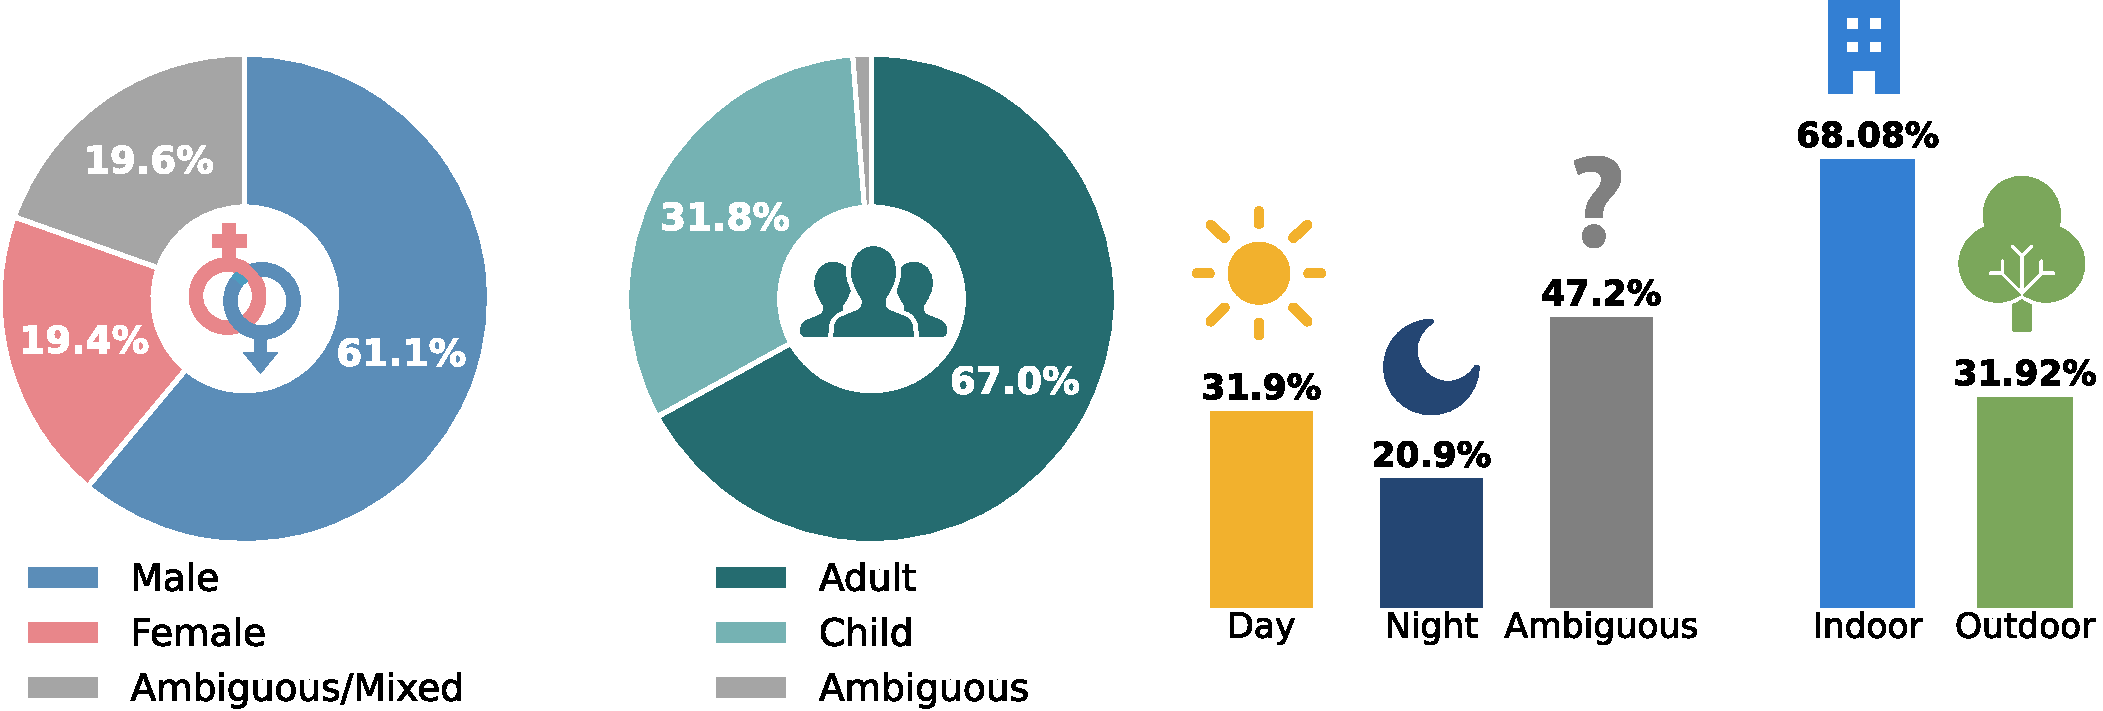
\includegraphics[width=\linewidth]{figures/dataset_demography.pdf}
    
  \caption{\textbf{Demography (aggressors and victims) and environment settings.} A$^3$Bench contains a larger proportion of male and adult participants among videos where demographic attributes are identifiable. For scene conditions, many clips are ambiguous in time of day, but among identifiable cases, slightly more aggressive clips occur during daytime than night, and most are captured in indoor environments.
}

  \label{fig:dataset_demograph}
\end{figure}

\begin{figure}[h!]
  \centering
  \begin{minipage}{0.64\linewidth}
    \centering
    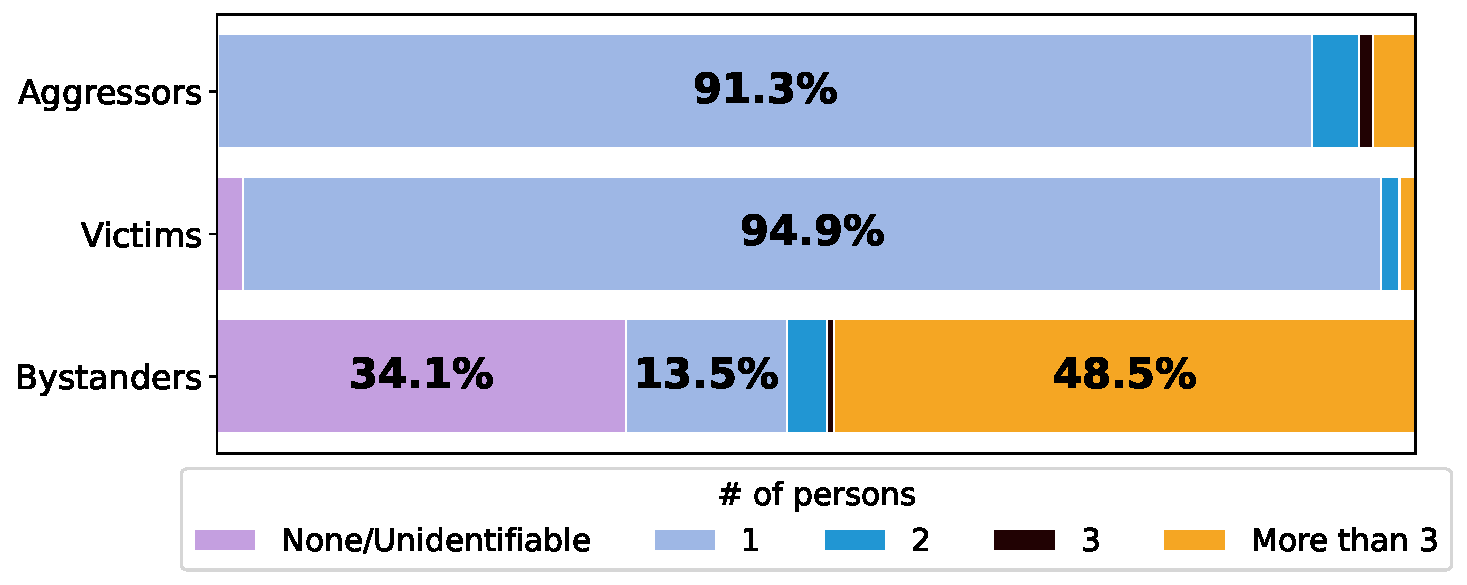
\includegraphics[width=\linewidth]{figures/role_distribution_by_video.pdf}
  \end{minipage}%
  \hfill
  \begin{minipage}{0.34\linewidth}
    \captionof{figure}{\textbf{Distribution of annotated roles per video.}
The role-count distribution is also skewed towards most clips containing a single identifiable aggressor and victim, while bystanders are more variable and often appear in larger groups.
}
    \label{fig:video_role_count}
  \end{minipage}
\end{figure}


\textbf{Question generation and distractor design:}
From the annotation corpus, we generate multiple-choice video question-answer pairs that function as controlled diagnostic probes for aggressive interaction understanding. Rather than only evaluating whether a model can recognize an action label, A$^3$Bench is designed to expose distinct failure modes in video-language models, including weak role grounding, poor action-participant binding, confusion between visible and relevant people, failure to model interaction directionality, and reliance on answer-choice priors.  The questions are organized into three tiers of increasing complexity: \textit{basic questions}, \textit{compound questions}, and \textit{detailed questions}. Figure~\ref{fig:teaser} illustrates representative examples from these three categories, and Figure~\ref{fig:question_type_category} reports their subcategories and overall distribution across the benchmark.

\textit{Basic questions} test whether a model can recover a single atomic attribute of the scene. These include primary action identification, where the model must recognize the aggressive action taking place; aggressor or victim identification, where the model must identify who performs the aggression or who is targeted; and role identification, where the model is given a person description and must assign the correct role, such as aggressor, victim, or bystander. These questions diagnose whether the model can localize individual actions and participant roles before requiring relational reasoning.

\textit{Compound questions} test whether a model can bind two scene attributes correctly. These include aggressor-victim, action-aggressor, and action-victim associations. Since each answer choice is only correct when all components are jointly correct, these questions diagnose whether models merely recognize visible actions or participants independently, or whether they can associate the correct action with the correct person and role.

\textit{Detailed questions} test whether a model can recover the full event structure of an aggressive interaction. These include aggressor-action-victim questions, which ask who did what to whom, and sequence verification questions, which require selecting the correct structured description of the interaction. These questions specifically diagnose failures in directionality, role distinction, and holistic event understanding, since a model must distinguish the aggressor from the victim and construct a coherent representation of the interaction rather than predict a participant-agnostic action category.


\begin{figure}[h!]
  \centering
  \begin{minipage}{0.64\linewidth}
    \centering
    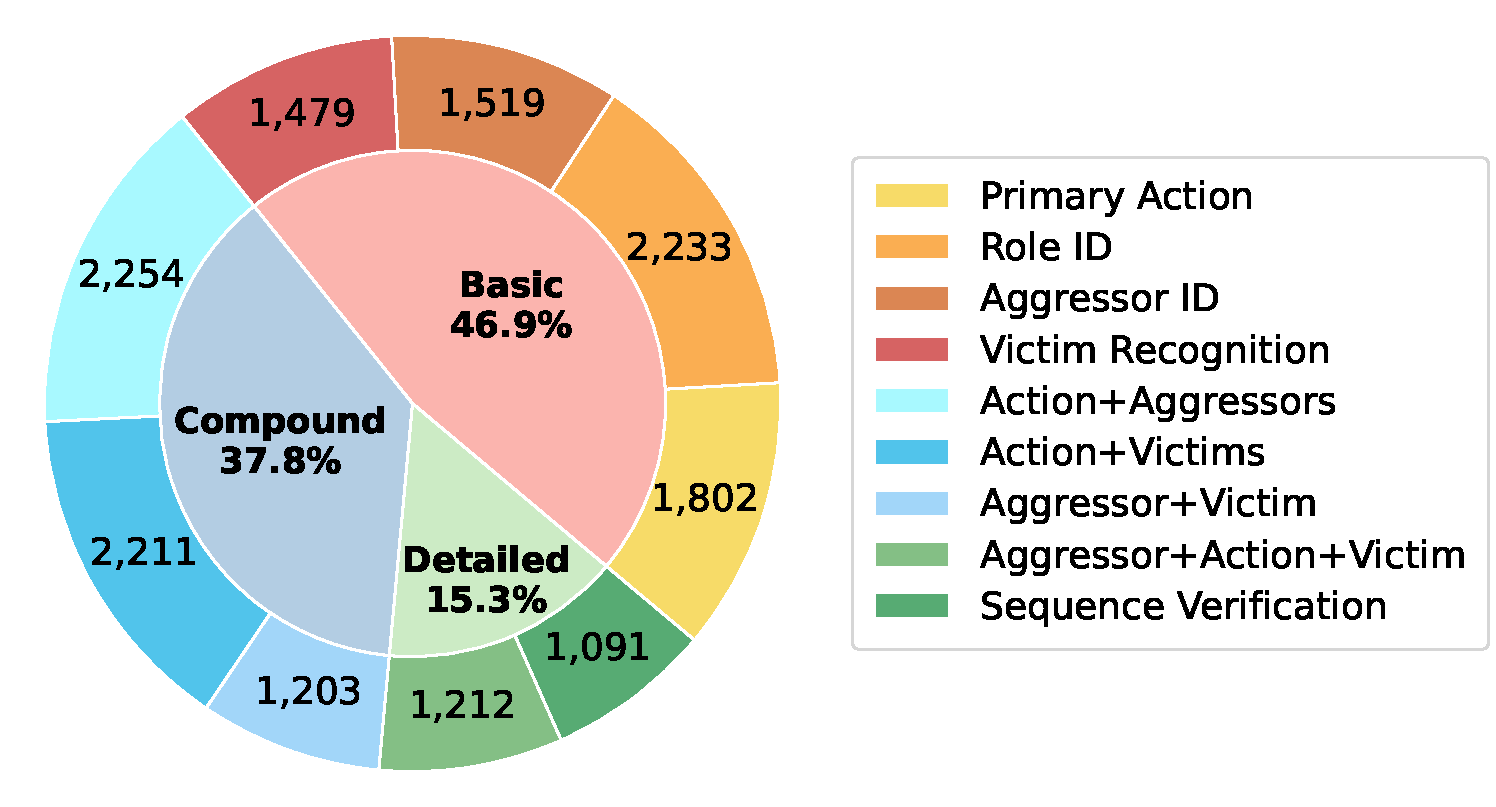
\includegraphics[width=\linewidth]{figures/category_distribution.pdf}
  \end{minipage}%
  \hfill
  \begin{minipage}{0.34\linewidth}
    \captionof{figure}{\textbf{Distribution of question types in A$^3$Bench.}
The benchmark contains three levels of questions with increasing association complexity: \textit{Basic} questions focus on single attributes; \textit{Compound} questions require associating two scene components; and \textit{Detailed} questions require full interaction understanding.
}
    \label{fig:question_type_category}
  \end{minipage}
\end{figure}


We design distractor choices as targeted diagnostic stress tests: they are visually plausible, semantically close to the correct answer, and tied to specific failure modes. \textit{Cross-video distractors} are sampled from real annotations of other clips, so incorrect options still contain natural actions, roles, and participant descriptions rather than synthetic or obviously invalid answers. \textit{Same-video distractors} use visible non-target participants from the queried clip, such as the victim or a bystander when asking for the aggressor, preventing models from relying only on visibility, saliency, or person presence. \textit{Role reversals and bystander substitutions} preserve much of the event content while swapping aggressor and victim roles or assigning bystanders to active roles, directly testing interaction directionality and the distinction between active participation and mere presence. \textit{Negation questions} include answers such as ``no aggressive action is taking place'' to test whether models verify visual evidence rather than assume aggression is present. \textit{Frequency-inverted distractors} are constructed so that each key distractor property, such as an action, role, or participant description, appears across multiple answer options, making marginal answer frequency uninformative. This forces models to reason over the complete aggressor-action-victim structure rather than selecting the option with the most common or familiar textual components.




\subsection{Benchmarked Models}

We evaluate MLLMs from \textbf{15} representative configurations on \textbf{A$^3$Bench} to assess their ability to perform aggressive action and association. All of our chosen models are trained on very large datasets with high-level video understanding. 

\noindent \textbf{General-Purpose Models.}
The evaluated models cover several recent open-weight MLLM families, including Gemma \cite{gemma4}, InternVideo \cite{internvideo2_5}, InternVL \cite{internvl2_5, internvl3, internvl3_5}, LLaVA-Video \cite{llavavideo}, Ovis \cite{ovis2_5}, Qwen-VL \cite{qwen-vl2_5, qwen3vl}, and VideoLLaMA \cite{videollama3}. These families differ in visual encoder design, video modeling strategy, instruction tuning, model scale, and reasoning behavior. 

\noindent \textbf{Reasoning and Prompted Variants.}
To investigate whether explicit reasoning improves aggressive action and association, we additionally evaluate reasoning-oriented variant of Qwen3-VL-8B \cite{qwen3vl} and enable reasoning-mode in Ovis2.5-9B \cite{ovis2_5}. We also evaluate InternVL3.5-8B \cite{internvl3_5} under two reasoning-style prompting settings: a detailed chain-of-thought (CoT) prompt and a Dream-of-Thoughts (inspired from \cite{navigatinghallucinations}) prompt. These variants encourage intermediate reasoning before producing a final answer, allowing us to test whether step-by-step inference helps models distinguish aggressors, victims, bystanders, actions, and scene context.


\subsection{Implementation Details, Evaluation Protocol, and Metrics}

All models are evaluated using their official implementations and released weights on a single NVIDIA RTX A6000 (48 GB) or A100 (80 GB) GPU. Qwen2.5-VL-72B-Instruct \cite{qwen-vl2_5} was run on the quantized version to fit in memory. We use a multiple-choice video question answering (VQA) protocol across all models: for each video-question pair, the model is prompted to select the most appropriate answer from the provided options. Depending on the question type and the size of the valid answer space, each question contains four to eight answer choices, including one correct answer and a set of diagnostic distractors. The position of the correct answer is uniformly shuffled across all questions to mitigate positional bias. This controlled evaluation setting enables fair comparison across models while directly measuring each model's ability to associate aggressive actions with the correct participants and roles. We report accuracy as the primary evaluation metric.
\YSR{no mention of train/test split?} \RA{No, since training free method, so no train set}


\begin{comment}
We also design distractor choices as targeted diagnostic stress tests. Each distractor type is constructed to be visually plausible, semantically close to the correct answer, and tied to a specific failure mode in aggressive action and association.
\begin{enumerate}
    \item \textbf{Cross-video distractors.} Incorrect answers are drawn from real annotations of other videos in the dataset. This ensures that distractors correspond to natural actions, roles, and participant descriptions rather than synthetic or obviously invalid choices. These distractors test whether models can distinguish the queried event from visually and semantically plausible alternatives.

    \item \textbf{Same-video distractors.} For person identification questions, we sample individuals with other roles who are visible in the same video. For example, when asking for the aggressor, the victim or a bystander may appear as an incorrect option. Because these individuals are genuinely present in the clip, the model cannot solve the question by simple visibility or saliency cues. This tests whether models can ground the queried role to the correct participant rather than selecting any visible person.

    \item \textbf{Role reversals and bystander substitutions.} For compound and sequence questions, we construct distractors by swapping the aggressor and victim roles. These choices preserve the same people and often the same action, but invert the relational structure of the event. This directly tests whether models understand the directionality of aggression rather than merely detecting the presence of the correct participants or action. We also place bystanders in active roles to test whether models can distinguish actual participation from mere presence in the scene.

    \item \textbf{Negation questions.} In many cases we use negation as the correct answer, such as ``no aggressive action is taking place''. These questions test whether models verify the visual evidence instead of relying on the benchmark prior that aggressive content is likely to be present. They therefore diagnose over-prediction of aggression and failure to reject unsupported relations.

    \item \textbf{Frequency-inverted distractors.} A key concern with multiple-choice evaluation is that models may exploit statistical regularities in answer text rather than ground responses in the video. To counteract such shortcuts, in Detailed questions, we use frequency-inverted distractor construction, where each distractor property appears across multiple options and marginal answer frequency is made uninformative. This forces the model to reason over the full aggressor-action-victim structure rather than selecting the option with the most common or familiar textual components.
\end{enumerate}
\end{comment}